\ifpdf
	\graphicspath{{3/pic/PNG/}{3/pic/PDF/}{3/pic/}}
\else
	\graphicspath{{3/pic/EPS/}{3/pic/}}
\fi

\chapter{Numerical methods for neutron transport}\label{chap:nte-methods}

As mentioned in the introductory chapter, we will focus on deterministic methods for solving the NTE, requiring proper
discretization of \eqref{eq1} and solution of the resulting system of algebraic equations. 
In the following sections, we review some of the most widely used (in author's opinion) semi-discretizations with respect to
energy, angle and spatial variables and finish this chapter with a general discussion on solving large sparse systems of
algebraic equations, resulting from the combination of semi-discretizations that are most suitable for our purposes. We
will focus on the fixed-source problem, whose solution is a neccessary part in practically all numerical methods for
solving the generalized eigenvalue problem \eqref{eq:critical}.

\myparagraph{Notation conventions}
Concerning fonts and subscripts/superscripts, we will generally use the following conventions (wherever exception will
be needed, it will be clearly stated):
\begin{itemize}
  \item $\mathbf{f}$ $\ldots$ column vector with numerical values ($\mathbf{f}\in\R[N]$ for some $N\in\mathbb{N}$)
  \item $f_n$ or $[\mathbf{f}]_n$ $\ldots$ components of $\mathbf{f}$
  \item $\mathbf{A}$ $\ldots$ matrix with numerical values ($\mathbf{A}\in\R[M\times N]$ for some $M,N\in\mathbb{N}$)
  \item $A_{ij}$ or $[\mathbf{A}]_{ij}$ $\ldots$ elements of matrix $\mathbf{A}$
  \item upshape $\mathrm{F}$ $\ldots$ vector function $\VV\to\R[N]$, $N\in\mathbb{N}$ 
  \item $f_n$ or $[\mathrm{F}]_n$ $\ldots$ components of $\mathrm{F}$ (we will not need to distinguish between
  components of $\mathrm{F}$ and $\mathbf{f}$ at the same place, so we use $f_n$ for both)
  \item $A$ or calligraphic $\mathcal{A}$ $\ldots$ in the context of an operator acting on some vector space $V$, usual
  letters will be used for transport operators introduced in previous chapter, while calligraphic letters for general  
  operators
%   \item $[A]_{ij}$ $\ldots$ sometimes we will use matrix operators acting on $\mathrm{F}\in V^N$; then 
%   $$
%   	[A \mathrm{F}]_{i} = \sum_{j=1}^N [A]_{ij} f_j
%   $$
  \item $s = \{c_k\}_{k=1}^N \equiv \{c_k\}_\idxset{N}$
  \item $\col s$ $\ldots$ column vector with entries $c_1,c_2,\ldots,c_N$
  \item $\diag s$ $\ldots$ diagonal matrix whose diagonal is given by elements of $s$
  \item $f_{(i)}$ $\ldots$ $i$-th iterate in an iteration process
\end{itemize}
So with this notation, we have, for instance, $\mathrm{F} = \col \{f_n\}_N$ with each $f_n$ being a function from some
space $V_n$.

\section{Approximation of energetic dependence}\label{sec:MG}

The continuous dependence on energy, $\psi = \psi(\cdot, E)$, is typically resolved by the so called \textit{multigroup
approximation}. In this approximation, the interval of neutron energies is divided as follows:
$$
\begin{multlined}
  \bigl[\Emin,\Emax] = \bigl[E^{G}-\dEh{G},E^{G}+\dEh{G}\bigr]\cup \ldots\\
  \ldots \cup \bigl[E^{g}-\dEh{g}, E^{g}+\dEh{g}\bigr] \cup \ldots \cup
  \bigl[E^1-\dEh{1},E^{1}+\dEh{1}\bigr],
\end{multlined} 
$$
and equations \eqrefs{eq1}{eq:nte3} are integrated over each energy group range 
\linebreak
\mbox{$\bigl[E^{g}-\dEh{g}, E^{g}+\dEh{g}\bigr]$}.
\begin{remark}
Note that the energy intervals (groups) are traditionally numbered in a descending order, i.e. a group with larger index
contains lower energies than a group with lesser index; also, the group index is traditionally placed in superscript. 
\end{remark}
The NTE \eqref{eq1} is thus transformed into a finite system of integro-differential equations, each
governing the flux of neutrons with energies within a particular range (in this context called \textit{group}):
\begin{equation}\label{eq:psi-MG}
\begin{multlined}
  \psi^g(\br, \bomega) = \frac{1}{\Delta E^{g}}\int_{g}\psi(\br, \bomega, E),\d{E} \equiv
  \frac{1}{\Delta E^{g}}\int_{E^g-\Delta E^{g}/2}^{E^g+\Delta E^{g}/2}\psi(\br, \bomega, E),\d{E},\\ g = 1, 2,\ldots
  G.
\end{multlined}
\end{equation} 
This conventional procedure leads to the following set of $G$ coupled neutron transport equations
\begin{equation}\label{eq:mg}
	\left\{
	  \begin{aligned}
      &T_G\{\psi^g\}_G = \{q^g\}_G,\\
      &\Dom{T_G} = \bigl\{\{\psi^g\}_G\in \bigl[\Hp(\XE)\bigr]^G,\ \psi^g\vert_{\pXE[-]} = 0,\ g = 1,\ldots,G\bigr\},
    \end{aligned}
  \right.\\[.2em]
\end{equation}
where
$$
	\XE := \{(\br,\bomega):\ \br\in \VV\subset\R[3], \bomega\in \Sphere\}
$$
is the 5-dimensional subspace of $X$ (i.e., the norm in $\Hp(\XE)$ is defined as
in \eqref{eq:Hp} but only using double integrals over $\VV\times\Sphere$) and analogously for $\pXE$.
The multigroup transport operator has the following form:
\begin{equation*}
\begin{gathered}
    T_G\{\psi^g\}_G = \left\{\left(A + \Sigma_r^g\right)\psi^g - \summ{g'=1,g'\neq g}{G}
    K^{gg'}\psi^{g'}\right\}_G,\\
    \bigl(\Sigma_r^g\psi^g\bigr)(\br,\bomega) = \sigma_t^g(\br)\psi^g(\br,\bomega) - \intA[']{\kappa^{g\sla
    g}(\br,\bomega\cdot\bomega')\psi^g(\br,\bomega')},\\ \bigl(K^{gg'}\psi^{g'}\bigr)(\br,\bomega) =
    \intA[']{\kappa^{g\sla g'}(\br,\bomega\cdot\bomega')\psi^{g'}(\br,\bomega')}
\end{gathered}
\end{equation*}
where the terms with superscript $g$ or $g'$ represent quantities suitably averaged over 
\mbox{$\bigl[E^{g}-\dEh{g}, E^{g}+\dEh{g}\bigr]$}, e.g. $K^{gg'}$ is (in theory) obtained as
\begin{equation}\label{eq:mg-kappa}
	\kappa^{gg'}(\br,\bomega\cdot\bomega') = \frac{\int_{g}\int_{g'} \kappa(\br,\bomega\cdot\bomega',E \sla
	E')\psi(\br,\bomega,E')\,\d{E'}\d{E}}{\int_{g}\psi(\br, \bomega', E)\,\d{E}}.
\end{equation}
It is customary to move the \textit{self-scattering} (diagonal) part of the
collision operator to the reaction operator. Since the reactions in which energetic distribution of both the incoming 
and outgoing neutrons lies within the same group are included in both $\sigma_t$ and $\kappa$  (compare equations
\eqref{eq:ddifxs} and \eqref{eq:st}), this transformation makes $\Sigma_r^g\psi^g$ represent the actual rate of neutron
removal from the group, while $K^{gg'}\psi^{g'}$ the rate of neutron addition to that group. Results about unique
solvability presented in previous chapter carry over to the multigroup setting by considering a counting measure on the
set $\{E^G,\ldots,E^1\}$ instead of the continuous Lebesgue measure $\d{E}$ \cite[Chap. XXI \S 2]{DautrayLions}.

\subsection{Multigroup data}
Although the multigroup system of neutron transport equations has a relatively simple form, finding an optimal grouping
of energies and determining the associated group-averaged coefficients is not an easy task in most practical
applications because of the highly complicated energetic dependence of nuclear processes, as illustrated by the typical
dependence of the (microscopic) fission cross-section of \isotope[235][92]{U} in the so-called resonance range of
energies and corresponding multigroup approximation in Fig. \ref{fig:xs}.
\begin{figure}[htp]
\begin{center}
  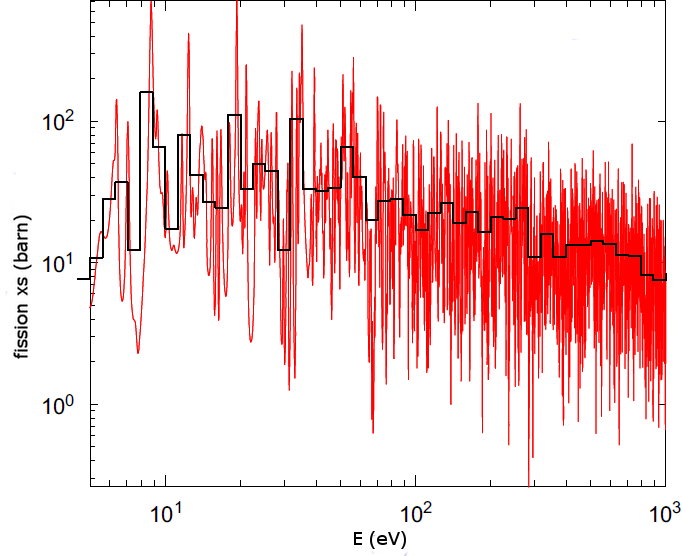
\includegraphics[scale=.4]{U235fg}
  \caption{Microscopic fission cross-section of U235}
  \label{fig:xs}
\end{center}
\end{figure}
Suitable approximation of the unknown exact solution in \eqref{eq:mg-kappa} is also highly non-trivial, albeit essential
for the success of the multigroup method. Even though an alternative to the finite-volume like approximation
\eqref{eq:psi-MG} has been proposed recently  in \cite{Douglass} -- using Galerkin projection of angular flux onto a
space of functions supported over subregions of the energy range (a finite-element like approach) --  the multigroup 
approximation still remains the most universally used approach to simplify the energetic dependence (see, e.g., 
\cite[Chap.~5]{Cacuci1} or \cite{Cho1}). However, we will not specifically address this issue and always assume that 
the multigroup coefficients appearing in the equations are given as input.
\begin{remark}{\textsc{Fission spectrum}}
In criticality problems, the set of multigroup data must include both parts of the collision kernel
$\kappa^{gg'}$, i.e. the cross-sections $\sigma_s^{gg'}$ and $\sigma_f^{gg'}$, as well as $\nu^{g'}$ and
$\chi^g$ (neutron yield from inelastic scattering, $\eta$, is usually absorbed into $\sigma_s$). Because of the rapid
decay of $\chi(E)$ for low energies (as neutrons are mostly emitted with high energies from fission) that are
nevertheless the most important for the cross-sections (as most interactions are likely to occur due to slowly moving
neutrons, at least in classical moderated reactors)\footnote{cf. \fref{fig:xs} and \fref{fig:spectrum} and notice the
different scaling on the horizontal axis}, there will typically be $\chi^g = 0$ for $g = G,G-1,\ldots,G-k$. The
group-discretized operator $F$ from \eqref{eq:FScrit} will therefore have a non-trivial null-space, leading ultimately
to a fully discrete generalized eigenproblem of type $\mat{A}\mat{x} = \lambda\mat{B}\mat{x}$ with singular $\mat{B}$.
\end{remark}


\subsection{Group source iteration}
A standard way of iterative solution of the multigroup system is the \textit{group source iteration}: for a given
initial approximation $\psi^g_{(0)}$, $g = 1,\ldots,G$, solve
\begin{myitemize}
  \item \textbf{for} i = 0,1,\ldots
  \begin{myitemize}
  \item \textbf{for} g = 1,\ldots,G
  \vspace*{-.5em}
	\begin{equation}\label{eq:MGGS}
		\left(A + \Sigma_r^g\right)\psi^g_{(i+1)} = \summ{g'\leq g-1}{} K^{gg'}\psi^{g'}_{(i+1)} + \summ{g' \geq g+1}{}
	  K^{gg'}\psi^{g'}_{(i)} + q^g
	\end{equation}  
 \end{myitemize}
\end{myitemize}
If we view the operator $T_G$ as a matrix operator acting on $\col \{\psi^g\}_G$, then we can interpret
this iteration as a Gauss-Seidel iteration for \eqref{eq:mg}, where $T_G$
has been split into its lower-triangular part $A + \Sigma_r^g - K^{gg'}$ ($g'\leq g$) and its upper triangular part 
$K^{gg'}$ ($g'> g$) and the lower triangular part is being inverted by forward substitution. Convergence of this scheme can become slow when the upper triangular part (representing neutron up-scattering
from lower energies to higher energies) is dominating. Therefore, when preparing the multigroup data, it is
advantageous to put an effort into finding such an energy grouping that minimizes the up-scattering (which is often
done in practice, as in e.g. \cite{mox-bench}).
\begin{remark}\label{rem:SI}
Here we assume that the
mono-energetic problem can be solved exactly. Approximations of angular dependence discussed in the following
section (like the $\SN$ method) may employ another iteration level to resolve angular
coupling of the within-group fluxes induced by collisions. This iteration is usually called just \textit{source
iteration} and can also become very slow if scattering of neutrons with given energy dominates their absorption (we will
return to this issue later in \sref{sec:SI}).
\end{remark}

Note that by employing the group source iteration, only a mono-energetic transport problem in group $g$ has to be
solved in each iteration, and if the differential part $A$ can be represented by a symmetric operator $\tilde A$ (as can be done for some of the second-order forms
described in \sref{sec:L2} or when suitable angular approximations like diffusion are being
used -- see \sref{sec:diffusion}), the problem would become symmetric with implications for efficient numerical
solution. In the remainder of this chapter, we will focus on the approximation of neutron flux in a single
group (index of which will be omitted), described by the corresponding within-group equation in which contributions from
other groups are encapsulated in the source term $\src$ (i.e., we will study the NTE on $\XE$). In order to simplify
notation, we will use just $X$ instead of $\XE$ when refering to the solution domain.

\section{Approximation of angular dependence}

Considerably larger number of methods have been proposed for approximating the angular dependence of neutron
flux. Many of them are still used and actively developed today as their characteristics make them more suitable for one
application area than other methods, which are preferred in different areas.

\subsection{Lattice calculations} \label{sec:lattice}
As a first example, we consider the class of
methods originally derived from the equivalent integral form of the NTE (see \sref{sec:advection}). Typical
representatives of this class are the method of collision probabilities or the method of characteristics (see e.g.
\cite{Cho2,Wu1,Hursin1,Petkov1,Sanchez1}). As the integral form of the NTE represents the global neutron balance over
the domain, the corresponding algebraic systems (obtained after spatial discretization) are full and
their solution demanding on computer resources. On the other hand, these methods quite naturally handle complex
geometries. Taking into consideration smaller geometric features of the domain, we are effectively coming from a
macroscopic scale to a mesoscopic range where the neutrons direction of motion as well as their kinetic energy become
more significant. High degree of spatial coupling and the requirement of fine resolution of angular and energetic
dependence does not make these methods suitable for whole-core reactor calculations.
However, these small-scale,
high-fidelity calculations\footnote{called \textit{lattice calculations} as they are typically performed on a single
representative subdomain of the core (one or several neighboring assemblies of fuel pins, or the fuel pin itself)
with reflective boundary conditions, simulating an infinite lattice of such subdomains} are indispensable for
generating appropriately averaged coefficients for the computationally more feasible larger scale calculations.
This \textit{spatial homogenization} and \textit{energy group condensation} (already mentioned in the previous
section), as these averaging procedures are traditionally called in nuclear engineering field, are employed by many existing whole-core simulators (see e.g.
\cite[Chap. 17]{Reuss1} or the review in first two sections of \cite{Sanchez7}). To simulate a long-term nuclear reactor
operation, it is furthermore neccessary to perform these procedures under varying physical conditions of the core and
generate many sets of averaged coefficients corresponding to these conditions.\comment{The code system
developed as part of author's involvement in the TACR project expects these coefficient sets on input, i.e., it is not
designed for lattice calculations.}

\vspace*{1em}
More suitable for whole-core calculations are methods derived from the integro-differential
version of the NTE, eq.
\eqref{eq1}, which lead to sparse algebraic systems. The most successful and well-established are the method
of discrete ordinates ($\SN$) and the method of spherical harmonics ($\PN$).
Both arise from applying in the
angular domain a classical well known approach for constructing finite numerical
approximations of PDEs. \comment{Although in the final code, we ultimately use the lowest order approximation that can
be obtained equivalently from both approaches (the neutron diffusion model) we will briefly introduce the main ideas behind the
$\SN$ and $\PN$ methods and expose their most important properties in the next two subsections.} In the two following
subsections, we will briefly introduce the main ideas behind the $\SN$ and $\PN$ methods and expose their most
important properties. These properties are generally known, but their origin in mathematical structure of the
approximate forms is mostly overlooked in literature (a few exceptions will be cited below and in the corresponding
appendices). 

We will also interpret both methods as restrictions of the same continuous NTE onto appropriate 
finite-dimensional subspaces of $\Hp[2](X)$. This is automatic in the case of the $\PN$ approximation (which is
basically a Galerkin method in angular domain with globally supported continuous basis functions), but has (as far as
the author knows) not been explicitely done for the $\SN$ approximation. Apart from showing both methods in the same light, this approach also allows to use properties
of the continuous transport operators to analyze the behavior of the approximate methods. We will illustrate it by demonstrating that the $\SN$ approximation doesn't 
preserve the rotational invariance property of the NTE characterized in \sref{sec:rotinv} while the $\PN$ approximation 
does. We will work in the context of the original first-order form of NTE, but this approach applies also when the
$\SN$ (or $\PN$) methods are used to approximate angular dependence in the second-order forms recalled in
\sref{sec:L2} (leading to coercive and bounded operator equations in the approximation subspaces). \comment{has also a
more useful consequence -- it allows to use properties of the continuous transport operators to analyze the behavior of the approximate methods. We will demonstrate it on the convergence analysis of the \textit{scattering source iteration}, a simple yet important method for practical use of the $\SN$ method\footnote{and remark that the same approach could be performed for the general multigroup source iteration described in previous section}. As a possible direction for future research, this approach could also be used to design new preconditioners, as outlined in a recent paper \cite{Kirby}.
}
\subsection{The $\SN$ method}\label{sec:1-SN}
The standard derivation of the $\SN$ method uses the collocation approach in which a set of directions
(\textit{ordinates}) $\omega = \{\bomega_m\}_{m=1}^{M}$ is chosen and the solution is approximated as:
\begin{equation}\label{eq:sn_approx} 
	\psi(\br, \bomega) \approx 
		\pw{\psi(\br,\bomega_m)}{if $\bomega = \bomega_m$ for $\bomega_m \in \omega$}
		   {0}{if $\bomega \not \in \omega$.} 
\end{equation}
Equation \eqref{eq1} as well as the boundary conditions \eqref{eq:nte2} or \eqref{eq:nte3} are then evaluated at these
$M = M(N)$ isolated directions. Notice that reflective (or albedo) boundary conditions place restrictions on the set of
ordinates as it should optimally contain both directions of each reflected pair (otherwise an interpolation would be
needed). For the traditional direction sets, we have $M = N(N+2)$ if the given problem does not possess any symmetries;
the method of discrete ordinates using such a number of directions is traditionally refered to as the method of 
discrete ordinates of order $N$, shortly $\SN$.

In order to evaluate the integral term on the right hand side of the equation, the set of directions is accompanied by a
corresponding set of weights $\{w_m\}_{m=1}^{M}$, together defining a quadrature of the sphere $\Sphere$. The
requirement of accurate evaluation of the integral term of eq.
\eqref{eq1} as well as accurate integration of the angular flux function over the sphere (to obtain the scalar flux)
constitutes the main guideline for the choice of directions and weights. We will return to this matter later in 
\sref{sec:DO}; for now it suffices to say that for three-dimensional problems without any symmetries, \mbox{$M = \left|\{\bomega_m, w_m\}\right| = \Oh(N^2)$} (with the
value of $M$ for typically used quadrature sets stated above).

To write  the final result of the $\SN$ approximation, let us first recall from \sref{sec:notation} that for a sequence
$s = \{c_k\}_\idxset{N}$, $\col s$ denotes the column vector with entries $c_1,c_2,\ldots,c_N$ and $\diag(s)$ the 
diagonal matrix defined by the elements of $s$. 
We define the vector functions representing $\SN$ solution and sources, respectively, as 
\begin{equation}\label{eq:sn_vars}
\Psi(\br) := \col\{\psi_m(\br)\}_{\idxset{M}},\quad
\mathrm{Q}_{S_N}(\br) := \col\{q_m(\br)\}_{\idxset{M}},
\end{equation}
the components of which are the fluxes and sources in ordinate directions
\begin{equation}\label{eq:sn_vecs}
\psi_m(\br) \equiv \psi(\br,\bomega_m), \quad q_m(\br) \equiv
q(\br,\bomega_m),\quad m = 1,\ldots, M.
\end{equation}

The $\SN$ approximation consists of the
following set of $M$ PDEs in spatial domain ($\br\in\VV$) \footnote{Differentiation and integration of vector functions
(such as the term $\pd{\Psi(\br)}{x}$ in eq. \eqref{eq:sn1}) is conventionally understood component-wise.}:
\begin{equation}\label{eq:sn1} 
\mat{A}_{S_N}^x\pd{\Psi(\br)}{x} + \mat{A}_{S_N}^y\pd{\Psi(\br)}{y} +
\mat{A}_{S_N}^z\pd{\Psi(\br)}{z} + \bigl[\sigma_t(\br)\mat{I} - \mathbf{K}_{S_N}(\br)\bigr]\Psi(\br) = \mathrm{Q}_{S_N}(\br),
\end{equation}
where $\mat{I}$ is the $M\times M$ identity matrix,
$$
	\mat{A}_{S_N}^x = \diag\{\Omega_{m,x}\}_{\idxset{M}},\ \mat{A}_{S_N}^y = \diag\{\Omega_{m,y}\}_{\idxset{M}},\
	\mat{A}_{S_N}^z = \diag\{\Omega_{m,z}\}_{\idxset{M}}.
$$
and
\begin{equation}\label{eq:SNK}
	\left[\mathbf{K}_{S_N}\right]_{m,n} = w_m \kappa(\cdot,\bomega_m\cdot\bomega_n),\quad
	\bomega_n,\bomega_m\in \omega,\ w_m\in \mathcal{W},\ 1 \leq m,n \leq M.
\end{equation}
Boundary conditions \eqref{eq:nte2} are easily taken into account as long as the ordinates set $\omega$ contains
directions in which $\psi_{\text{in}}$ is specified:
\begin{equation}\label{eq:bc_sn}
	\psi_m(\br) = \psi_{\text{in}}(\br, \bomega_m)\quad \br\in\pV, \ \bomega_m\cdot\bn < 0
\end{equation}	
while (as already mentioned above), the conditions of type
\eqref{eq:nte3} require that for each $\bomega_m\in\omega$, 
$$
	\bomega_m - 2 \bn (\bomega_m \cdot \bn) \in \omega.
$$ 
After solution vector $\Psi(\br)$ is computed, the
important physical quantities (scalar flux, neutron current) can be obtained directly from their definition \eqref{eq:scalar_flux}
\eqref{eq:bJ} using the quadrature formula, e.g.
\begin{equation}\label{eq:scalar_flux_sn}
\begin{aligned}
	\phi(\br) &= \intA{\psi(\br,\bomega)}\\
	 &= \sum_{m=1}^{M} w_m \psi(\br,\bomega_m) = \sum_{m=1}^{M} w_m \psi_m(\br), \quad
	\br\in \overline\VV,\ \bomega_m\in \omega,\ w_m\in \mathcal{W}.
\end{aligned}
\end{equation}

\subsubsection{Structure of the $\SN$ approximation}
\myparagraph{Advection}
Equation \eqref{eq:sn1} represents a system of advection-reaction equations, each with constant advection field given by
the matrices $\mat{A}_{S_N}^x, \mat{A}_{S_N}^y, \mat{A}_{S_N}^z$. We can see that it has a form of a decoupled
hyperbolic system, having $M$ unique plane-wave solutions propagating in directions $\{\bomega_m\}_{\idxset{M}}$. A
plane-wave propagating in direction $\mat{R}^T\bomega_m$, where $\mat{R}$ is the matrix representation of rotation
$\mathcal{R}\in \mathrm{SO}(3)$, will be a solution to the $\SN$ equations only if $\mat{R}^T\bomega_m \in \omega$. From
this observation, we can already see that the fundamental property of rotational invariance (in case of rotationally
invariant input data, see \sref{sec:rotinv}) is lost when approximating the continuous NTE by a finite $\SN$ system.
After interpreting the $\SN$ approximation as a projection of the continuous NTE onto an $\SN$ subspace, we will see
that this is a consequence of the form of the projection operator itself (and thus cannot be removed, for instance, by
considering the second-order forms of the NTE as a basis for the $\SN$ approximation).

In practice, this undesirable property manifests itself in the form of so-called ``ray effects''. As a consequence of
radiation propagating in a finite set of distinct directions, there will remain under-treated regions of the phase
space, while other regions will receive more radiation in order to satisfy the global balance. This leads to spurious spatial oscillations
of scalar flux (\textit{ray effects}), which become more pronounced as the spatial discretization is refined.
This issue is somewhat ameliorated when strong scattering is present (as it increases the coupling of the equations,
though it also makes them more difficult to solve numerically), but its true nature shows that the only systematic way
of reducing ray effects in the framework of the $\SN$ method is to increase the number of ordinates (especially when
trying to reduce spatial discretization errors by using finer mesh). Being arguably the biggest issue of the $\SN$ approximation, various more practical
remedies have been proposed in literature (which, as expected, typically sacrifice some properties of the $\SN$
approximation), see e.g. \cite{Li1} and the references therein.

\myparagraph{Collisions}
As we can see from \eqref{eq:SNK}, the term $\mathbf{K}_{S_N}\Psi$ induces full unknown coupling. In order to recover 
sparsity (and also facilitate the use of efficient constant-advection solvers based on explicit marching in the
advection  direction), the so-called  \textit{source iteration} (SI) \index{SI|see{source iteration}} is utilized, in which the system \eqref{eq:sn1} is
fully decoupled by moving $\mathbf{K}_{S_N}$ to the right. Each equation is solved separately using any method suitable for an advection-reaction PDE with constant
advection vector, using $\psi_m$ from previous iteration to evaluate $\mathbf{K}_{S_N}\Psi$. Classical iteration methods
like Jacobi and Gauss-Seidel are typically used to update $\Psi$ during the iteration process; e.g. the Jacobi scheme 
gives the iteration
\begin{equation}\label{eq:SI}
	\mat{A}_{S_N}^x\pd{\Psi_{(i+1)}}{x} + \mat{A}_{S_N}^y\pd{\Psi_{(i+1)}}{y} +
	\mat{A}_{S_N}^z\pd{\Psi_{(i+1)}}{z} + \sigma_t\mat{I}\Psi_{(i+1)}= \mathbf{K}_{S_N}\Psi_{(i)} +
	\mathrm{Q}_{S_N},\ 
	i = 0,1,\ldots
\end{equation}
for given initial approximation $\Psi_{(0)}$. We will return to the convergence properties of this iteration in
\sref{sec:SI}

\subsubsection{Projection form of the $\SN$ approximation}
To provide a direct comparison with the $\PN$ approximation presented in the
following section and a link to the continuous NTE, we will now formulate the $\SN$ method as a projection
onto an appropriate approximation subspace.%
\comment{
As motivated in \cref{chap:nte-review}, we would like to continue with approximating generalized solutions of the NTE, for which the
classical view of the $\SN$ approximation relying on extracting pointwise values on the sphere is not appropriate. We
can overcome this problem by formulating the $\SN$ method using a finite-volume approach on the sphere. 
}
To this end, let us consider an arbitrary $\SN$ approximation of a fixed source problem with homogeneous inflow boundary
conditions, specified by the given set of ordinates $\omega = \{\bomega_m\}_{\idxset{M}}$ and a corresponding set of
quadrature weights \mbox{$\mathcal{W} = \{w_m\}_{\idxset{M}}$}. 
For each $\bomega_m\in\omega$, we define a patch $\Delta\bomega_m$ on the sphere with (spherical) area $w_m$ (see
\fref{fig:element} where the patch would correspond to the shaded area and $\Delta\bomega_m = \abs{\d{\bomega}}$). This
construction requires 
$$
	\sum_{m=1}^M w_m = \mu(\Sphere) = 4\pi\quad \mbox{ and }\quad  w_m > 0, \ \, 1 \leq m \leq M,
$$
which is satisfied by most discrete ordinates quadrature sets in use\comment{\footnote{although we note that one of the
first and most widely used quadrature sets, Carlson's \textit{level-symmetric} set, allows negative weights when $N > 20$  (e.g.
\cite[Sec. 8.5.1]{Cacuci1})}}. Let $f\in V$, where $V$ can in general be some function space ensuring existence of
unique solution of the NTE (see \sref{sec:fixed-source} for examples). To facilitate the comparison with the $\PN$ method, we
will specifically consider the Hilbert space $V = \Lp[2](X)$. 
\comment{
and denote by $V_0$ the definition domain of the transport operator with
vanishing inflow boundary conditions:
$$
	V_0 = \{\psi\in \Hp[2](X),\ \psi\vert_{\pX[-]} = 0\} \subset \Lp[2](X).
$$
}  
Taking into account the definition of the $\SN$ unknowns by \eqref{eq:sn_vars}, let us define a mapping that
transforms the function $f$ to a spatial vector function $\mathrm{F}$ as:
 \begin{equation}\label{eq:map_SN_inv}
	\PihSN f = \col\left\{f(\cdot,\bomega_m)\right\}_{\idxset{M}}. %\equiv \col\left\{f_m(\cdot) \right\}_{\idxset{M}}.
	\footnote{We implicitly include in this mapping the orthogonal projection onto a dense subspace of $V$
comprising functions that are (as functions of $\bomega$) continuous at $\bomega_m\in\omega$ (this is a neccessary
technical step circumventing the problem of pointwise evaluation of functions $f(\cdot,\bomega) \in \Lp(\Sphere)$).} 
\end{equation}%
\comment{(more generally, we can find a dense
subspace $D\in \Lp[\Sphere]$ such that for each equivalence class $[f]\in D$, the linear functional $E_{\bomega_m} : [f] \mapsto
\hat f(\bomega_m)$, $\hat f \in [f]$ is linear and continuous on $D$ for each $\bomega_m\in\omega$; see}
%
Corresponding to it is the mapping which produces a function in $V$ from a vector function 
\mbox{$\mathrm{F}(\br) = \colset{f_m(\br)}{\idxset{M}}$}:
\begin{equation}\label{eq:map_SN}
\PiSN: \mathrm{F} \mapsto f\in V_{S_N},\quad
\bigl(\PiSN \mathrm{F}\bigr)(\br,\bomega) = \sum_{m=1}^M f_m(\br)\imath_m(\bomega),\quad
\left.\bigl(\PiSN\mathrm{F}\bigr)\right\vert_{\pX[-]} = 0
\end{equation}
where $\imath$ is the indicator function of the patch $\Delta\bomega_n$:
\begin{equation}\label{eq:indicator}
\imath_m(\bomega) = \pw{1}{if $\bomega \in \Delta\bomega_m$}{0}{otherwise.}
\end{equation}
Here we introduced $V_{S_N}\subset\Dom{L-K} \subset V$ as a subspace of a space of functions that are (as functions of
$\bomega$) piecewise constant on $\Sphere$ and satisfy the homogeneous inflow boundary condition\footnote{Note that an
analogous mapping could be defined for non-homogeneous boundary conditions and used in a lifting argument of type \eqref{eq:lifting} to convert
a nonhomogeneous boundary value problem to the one analyzed here.}. With these two
mappings, we can now rewrite the $\SN$ system \eqref{eq:sn1} in terms of the transport operators from eq.
\eqref{eq1op}:
\begin{equation}\label{eq:sn_op}
	\PihSN (\op{L} - \op{K}) \PiSN \Psi = \mathrm{Q}_{S_N},
\end{equation}
or, incorporating the definition of the $\SN$ variables \eqref{eq:sn_vars} by operator $\PihSN$, as
\begin{equation}\label{eq:sn_op2}
	\PiSN \PihSN (\op{L} - \op{K})\PiSN \PihSN \psi = \PiSN \PihSN q
\end{equation} 
with $\psi, q \in V$. Finally, we can see from \eqref{eq:map_SN_inv} and \eqref{eq:map_SN} that when $\PihSN$ is
restricted to $V_{S_N}$, $\PiSN\PihSN = I_{S_N}$ (identity on $V_{S_N}$) and thus the linear operator
$$
	\Projop[S_N] := \PiSN\PihSN,
$$
self-adjoint on $V$, is an orthogonal projection $V\to V_{S_N}$. The $\SN$ system \eqref{eq:sn1} can
therefore be written as
\begin{equation}\label{eq:sn_op3}
	\Projop[S_N] (\op{L} - \op{K})\Projop[S_N] \psi = \Projop[S_N] q,
\end{equation}
that is, as a restriction of the original continuous NTE onto $V_{S_N}$. \comment{(which, for the case $V = \Hp(X)$,
we will write as $\Hp_{S_N}(X)$)}

It is worth noticing that even though the systems \eqref{eq:sn_op}
and \eqref{eq:sn1} (with \eqref{eq:sn_vars} and \eqref{eq:sn_vecs}) are equivalent, the interpretation of the
solution of \eqref{eq:sn_op} is different from the point-wise approximation \eqref{eq:sn_approx}. The interpretation as
a piecewise constant (w.r.t. to $\bomega$) function over the ordinate patches is more natural, however, as it for
example directly leads to the scalar flux definition \eqref{eq:scalar_flux_sn}.
 
The $\SN$ method is sometimes described as an ``discretization by by delta functions'' \cite[p.133]{Chang}.
We remark that by using this kind of approximation to define the operators $\PihSN$ and $\PiSN$ (and supposing we
could overcome all the technical issues associated with a rigorous use of Dirac delta distribution), we would not be able to
put \eqref{eq:sn1} into an equivalent form involving only the original continuous operators as in \eqref{eq:sn_op}
because of the collision integral. It is also illustrative to write the weak form of eq. \eqref{eq:sn_op3}.  
Using symmetry of $\Projop[S_N]$, we obtain 
\begin{equation}\label{eq:SN_weak}
	\langle (\op{L}  - \op{K})\Projop[S_N] \psi, \Projop[S_N] \varphi \rangle = \langle q, \Projop[S_N]
	\varphi \rangle\quad \forall \varphi\in V. 
\end{equation}
This is a system that we would obtain if we approximated the directional dependence of the NTE by the
well-known discontinuous Galerkin (DG) method \index{DG|see{discontinuous Galerkin method}} with piecewise constant shape functions
generating $V_{S_N} = \Rng \Projop[S_N]$ (and imposing boundary conditions in a strong sense, i.e. by restricting the
approximation space). Note that in Cartesian coordinate system, there are no derivatives with respect to $\bomega$ in
the NTE, so that no jump terms arise at patch boundaries.
 
\subsubsection{Convergence of source iteration} \label{sec:SI}
Having established the connection between the fully continuous NTE in a Hilbert space $V$ and its $\SN$
approximation in $V_{S_N} \subset V$, we can now use properties of operators $L$ and $K$ to
investigate convergence of the source iteration in the discrete ordinates approximation. To this end, let us first write
\eqref{eq:SI} as an iteration on $V$:
$$ 
	\Projop[S_N] \op{L} \Projop[S_N] \psi_{(i+1)} = \Projop[S_N] \op{K} \Projop[S_N] \psi_{(i)} +  \Projop[S_N] q,\quad i =
	0,1,\ldots 
$$
(assuming given $\psi_{(0)} \in V$). The corresponding weak form is 
\begin{equation}\label{eq:SISN}
	\langle \op{L} \Projop[S_N] \psi_{(i+1)}, \Projop[S_N] \varphi \rangle = \langle \op{K}\Projop[S_N] \psi_{(i)} + q,
	\Projop[S_N] \varphi \rangle\quad \forall \varphi\in V,\quad i = 0,1,\ldots. 
\end{equation}
Again, this is just a restriction to $V_{S_N}$ of the following iteration in $V$:
\begin{equation}\label{eq:SIhilbert}
	\langle \op{L} \psi_{(i+1)}, \varphi \rangle = \langle \op{K} \psi_{(i)} + q, \varphi \rangle \quad \forall
	\varphi\in V \quad i = 0,1,\ldots.
\end{equation}

Egger and Schlottbom \cite{Egger} used Banach fixed point theory to the iteration \eqref{eq:SIhilbert} to show that the 
mapping $$ \mathcal{T}_q : u \mapsto L^{-1}K u + \L^{-1} q, \quad q \in \Lp(X)$$ is contractive for all $1
\leq p \leq \infty$ provided that conditions equivalent to those of Theorem \ref{thm1} (i.e., subcriticality
conditions) hold. With this result, the authors show well-posedness of Problem \ref{prb:1} (existence of
unique solution with continuous dependence on input data). 
They also exhibit the contraction factor (in our notation where $c$ and $d$ have been
defined in \eqref{eq:c} and \eqref{eq:d}, respectively) 
\begin{equation}\label{eq:contraction_factor}
	\rho_p = 1 - e^{-C_p}, \quad C_p = \frac{1}{p}\norm[{\Lp[\infty](X)}]{c\sigma_t\ell} +
	\frac{p-1}{p}\norm[{\Lp[\infty](X)}]{d\sigma_t\ell}, \quad 1 \leq p \leq \infty
\end{equation}
where $\ell = \ell(\br,\bomega)$ is the length of the characteristic line segment passing through $\br$ in the
direction $\bomega$, which we assume to be bounded and such that
$$
	\forall \bomega \in \Sphere\ \exists s_0:\ \, 0 < s_0 < \ell(\br,\bomega)\ \mbox{ and }\ \br_0 = \br - s_0 \bomega \in
	\pX[-]
$$
(see \fref{fig:trepka} in \sref{sec:advection}).
As the contraction property
$$
\exists \rho \in [0, 1): \norm[V]{\mathcal{T}_q\, u_1 - \mathcal{T}_q\, u_2} \leq \rho \norm[V]{u_1 - u_2}\quad
\forall u_1,u_2 \in V $$
holds also for any $u_1,u_2\in V_{S_N} \subset V$, we immediately get the convergence result for the $\SN$ source
iteration \eqref{eq:SISN}. 
\begin{theorem}\label{thm:3}
	For any $\psi_{(0)} \in V_{S_N}$, the sequence of iterates $\{\psi_{(i)}\}_{i=1}^{\infty}$ of the iteration
	\eqref{eq:SISN} converges to the unique solution $\psi^*$ of equation \eqref{eq:SN_weak} with $q \in V(X)$. 
	Moreover, 
	$$
		\norm{\psi_{(i)} - \psi^*} \leq \frac{\rho^{i}}{1-\rho} \norm{\psi_{(1)} - \psi_{(0)}},\quad
		\norm{\psi_{(i)} - \psi^*} \leq \frac{\rho}{1-\rho} \norm{\psi_{(i)} - \psi_{(i-1)}}.
	$$   
\end{theorem}

\begin{remark}[\textsc{Multigroup case}]\label{rem:MG}
	This approach is readily extended to the energy-dependent case once we recognize that the multigroup system
	\eqref{eq:mg} is again a restriction of the continuous NTE to a subspace of piecewise constant functions with respect
	to energy, using $\Projop[G] := \PiG\PihG$ where
	$$
		\PihG\psi = \left\{\frac{1}{\Delta E^{g}}\int_{g}\psi(\cdot,\cdot,E)\,\d{E}\right\},\quad
		\PiG\{\psi^g\} = \sum_{g=1}^G \psi^g(\cdot,\cdot)\imath_g(E).
	$$
	The above results then apply to the Jacobi version of iteration \eqref{eq:MGGS}, while the Gauss-Seidel form
	could be analyzed by splitting the continuous transport operator as 
	$$
		T = L + K_\downarrow + K_\uparrow,
	$$
	with
	$$
	\begin{aligned}
		K_\downarrow\psi(\br,E) &= \intE[']{E \leq E'}{}{
		\intA[']{\kappa(\br,\bomega\cdot\bomega',E\sla E')\psi(\br,\bomega',E')}},\\
		K_\uparrow\psi(\br,E) &= \intE[']{E > E'}{}{
		\intA[']{\kappa(\br,\bomega\cdot\bomega',E\sla E')\psi(\br,\bomega',E')}}.
	\end{aligned}
	$$
\end{remark}

\myparagraph{Source iteration under diffusive conditions}
Placing ourselves in the $\Lp[2](X)$ setting and noticing that in the
monoenergetic case in isotropic medium, $c = d$, the contraction factor \eqref{eq:contraction_factor} becomes
$$
	\rho_2 = 1 - e^{-\norm[{\Lp[\infty](X)}]{c\sigma_t\ell}}
$$
and we can see that $\rho_2$ gets closer to $1$ and the convergence rate deteriorates as the scattering becomes the
dominating collision event and the size of the domain gets larger. This means that the \textit{escape probability} of neutrons gets lower and neutrons diffuse
through the domain for a long time until they get absorbed (note that if we assume non-fissioning domain with $\sigma_f
= 0$ and neglect inelastic scattering, $c \to 1$ with fixed $\sigma_t$ implies $\sigma_a \to 0$, cf.
\eqref{eq:scattering_ratio} and \eqref{eq:st}). Such conditions
are referred to as \textit{diffusive conditions}. By classical asymptotic analysis (see e.g.
\cite{Larsen1} or the overview \cite{AdamsIdea} and references therein), the solution of the diffusion approximation (discussed
later in \sref{sec:dif}) tends to the solution of the NTE under such conditions. More precisely, 
``diffusivity'' of the medium is characterized by a small parameter $\varepsilon \ll 1$ such that $\varepsilon\to 0$ 
reflects the properties described above. The parameter is also defined in such a way that when the terms of the NTE are 
scaled by $\varepsilon$ and $\varepsilon \to 0$, the diffusion equation \eqref{eq:dif} is obtained up to terms of
order $\Oh(\varepsilon^3)$. Hence, in cases when the source iteration converges slowly, it makes sense to 
\textit{precondition} it by the solution of the diffusion problem, which is known as the \textit{diffusion synthetic
acceleration of SI}. For more details, we refer to \cite[Chap. 1]{Azmy1} or \cite[Sec. III]{Adams} (where also
convergence characteristics of the discrete ordinates source iteration similar to Thm. \ref{thm:3} were obtained for
homogeneous infinite medium by means of Fourier analysis).


\comment{
Writing the iteration in the form
$$
\PihSN \op{L} \PiSN  \Psi_{(i+1)} = \PihSN \op{K}_{S_N} \PiSN \Psi_{(i)} + \mathrm{Q}_{S_N},
$$
we can see that propert It can be shown by Fourier analysis that
in an infinite homogeneous medium, the iteration \eqref{eq:SI} suppresses those Fourier modes with wavelengths  see also Remark \ref{rem:SI}).
\cite[Chap. 1]{Azmy1}, or \cite[Sec. II.A]{Adams})
}


To summarize this subsection, we have shown that the traditional $\SN$ method that the weak form
of the $\SN$ approximation corresponds to the discontinuous Galerkin approximation in the angular domain. The $\PN$ method represents the continuous Galerkin approach.

\subsection{The $\PN$ method}\label{sec:PN}

The system of $\PN$ equations has been originally derived using the weighted residuals method in the angular domain,
whereby the angular flux is expanded into infinite series of functions of $\bomega$ that span a
complete basis on the unit sphere, the continuous neutron transport equation \eqref{eq1} is multiplied by each member of
the basis in turn and integrated over the sphere. The properties of the basis functions are then used to derive
equations for the expansion coefficients. Only a finite number of expansion terms is considered to allow practical computation.
Usually, the expansion is truncated to a finite length of $K = K(N)$ terms\footnote{The length of the expansion $K$
should not be confused with the operator $K$ introduced in the previous section; it will be always clear from context 
which meaning the letter $K$ currently has.} by setting all expansion coefficients with higher index to 0 (although there exist alternative closure methods that may have favorable properties in certain situations, see e.g.
\cite{Frank0}). Then we speak of the $\PN$ approximation:
\begin{equation}\label{eq1.1}
  \psi(\br,\bomega) \approx \sum_{k=1}^{ K} \phi_k(\br) \varphi_k(\bomega).
\end{equation}
A natural function space to support this procedure is the Hilbert space of
square-integrable functions on the sphere $\Lp[2](\Sphere)$, equipped with the inner product
\begin{equation}\label{eq:s2_ip}
	(u, v)_{\Lp[2](\Sphere)} = \intA{u(\bomega) {v(\bomega)}}.
\end{equation}
We will therefore assume \mbox{$\psi(\cdot,\bomega)\in\Lp[2](\Sphere)$} (as is the case, e.g., when 
$\psi\in\Hp[2](X)$).

Note that \eqref{eq1.1} has the same form as the approximation 
$$
	\psi \approx \PiSN\PihSN\psi = \Projop[S_N]{\psi},
$$
where $K = M$ and $\phi_k = \imath_k$, $1 \leq k \leq K$ have been used (as can be seen from relations
\eqrefs{eq:map_SN_inv}{eq:indicator}). The system of spherical basis functions that were used in the original $\PN$
method is the system of \textit{spherical harmonic functions} (shortly \textit{spherical harmonics}, App. \ref{app:SH}).
We will consider here the real system (whose elements are sometimes called \textit{tesseral spherical harmoncs}) as it is more convenient
for practical purposes than the equivalent complex system (which appears to be more traditional in nuclear engineering 
literature, e.g. \cite[Sec. 9.7]{Stacey1}, \cite[Sec. 14.4]{Reuss1}), \cite[Chap. V]{Stammler}). Spherical harmonics
form a complete orthonormal system on $\Lp[2](\Sphere)$ with respect to the inner product \eqref{eq:s2_ip} (or its Hermitian 
variant when complex spherical harmonics are used) and simplify the algebraic manipulations needed to arrive at the 
conditions for coefficients $\phi_k$ (called \textit{angular moments}). 

In one dimension, spherical harmonics reduce to 
Legendre polynomials and $ K(N) = N$.
For general three-dimensional problems, there are $2n + 1$ linearly independent spherical harmonics for each degree $n$ 
and 
$$ 
	K(N) = \sum_{n=0}^{N} 2n + 1 = (N+1)^2.
$$
%
The approximation \eqref{eq1.1} is usually rewritten as a double sum
\begin{equation}\label{eq:pn_approx}
	\psi(\br,\bomega) \approx \sum_{k=1}^{ K} \phi_k(\br)\Y{k}{}(\bomega) \equiv
	\suma[n]{0}{N}\suma[m]{-n}{n}\angmom{n}{m}(\br)\Y{n}{m}(\bomega)
\end{equation}
where $\Y{n}{m}(\bomega)$ is the spherical harmonic function of degree $n$ and order $m$
and in the first term on right, we consider the single index $k$ ($1 \leq k \leq  K$) that covers all the combinations of $n$ and $m$ ($0 \leq n \leq N$, $-n\leq m \leq n$) appearing in the second term. We finally arrive at a system of $ K$
partial differential equations in spatial domain which is of comparable size as the system of $\SN$ equations and has the following form:
\begin{equation}\label{eq:pn1}
	\mat{A}^x_{P_N}\,\pd{\Phi(\br)}{x} + \mat{A}^y_{P_N}\,\pd{\Phi(\br)}{y} + \mat{A}^z_{P_N}\,\pd{\Phi(\br)}{z} +
	\bigl[\sigma_t(\br)\mat{I} - \mathbf{K}_{P_N}(\br)\bigr]\Phi(\br) = \mathrm{Q}_{P_N}(\br),
\end{equation}
where 
\begin{equation}\label{eq:pn_vectors}
	\Phi(\br) = \col\left\{\phi_k(\br)\right\}_{\idxset{K}} \ \text{ and }\ 
	\mathrm{Q}_{P_N}(\br) = \col\left\{q_k(\br)\right\}_{\idxset{K}}
\end{equation}
are, respectively, the vector functions of angular flux
moments and angular source moments.
The
Galerkin procedure results in their special form
\begin{equation}\label{eq:pn_angmom}
	\phi_k = (\psi, \Y{k}{})_{\Lp[2](\Sphere)},\quad q_k = (q, \Y{k}{})_{\Lp[2](\Sphere)};
\end{equation}
Using again the double index ($k = {}_n^m$) and the form of spherical harmonics with $n = 0,1$, we also obtain a direct
correspondence of the first four moments and the physically important quantities defined in \sref{sec:qoi}:
$$
	\phi = \sqrt{4\pi}\angmom{0}{0},\quad \bJ = \sqrt{\frac{4\pi }{3}}\, [\angmom{1}{1}, \angmom{1}{-1}, \angmom{1}{0}]^T.
$$


In view of \eqref{eq:pn_approx} and the completeness and orthogonality properties of spherical harmonics,
\eqref{eq:pn_angmom} also shows that the angular flux in the $\PN$ method is actually approximated by its orthogonal
projection onto the finite-dimensional subspace $\Lp[2]_K(\Sphere)\subset\Lp[2](\Sphere)$:
\begin{equation}\label{eq:PN_proj}
	\psi \approx \Projop\psi, \quad \Projop\psi(\cdot,\bomega) := \sum_{k=1}^{ K}\ips{\psi}{\Y{k}{}} \Y{k}{}(\bomega).
\end{equation}

\subsubsection{Operator form} \label{sec:pn_op}
It is illustrative to put the $\PN$ system \eqref{eq:pn1} into a form involving the transport operators from
eq. \eqref{eq1op}.
In order to do so, let us define mappings that take the vector function $\Phi(\cdot)$ to angular
flux $\psi(\cdot,\bomega)\in\Lp[2]_K(\Sphere)$ and vice versa. The general operators realizing this operation for the
case $\mathrm{F} = \Phi$ and $f(\bomega) = \psi(\cdot,\bomega)$, respectively, are
\begin{equation}\label{eq:pn_op_def}
\bigl(\PiPN\mathrm{F}\bigr)(\cdot,\bomega) := \sum_{k=1}^{ K} f_k(\cdot)\Y{k}{}(\bomega), \quad
\PihPN f = \col \left\{(f, \Y{k}{})_{\Lp[2](\Sphere)}\right\}_{\idxset{K}}.
\end{equation} 
Using \eqref{eq:pn_angmom}, \eqref{eq:pn_vectors} and \eqref{eq:PN_proj}, we can see that 
$$
\PiPN\Phi = \PiPN\PihPN \psi = \Projop\psi.
$$ 
Notice that when restricted to the space of functions that (as functions of 
$\bomega$) can be expressed as linear combination of spherical harmonics up to degree $N$, $\PihPN = \PiPN^{-1}$  (which
is equivalent to $\Projop[P_N]$ being a projection). 
The operator form of the $\PN$ system is thus
\begin{equation}\label{eq:pn_op}
	\PihPN (L-K) \PiPN\Phi = \mathrm{Q}_{P_N} = \PihPN q
\end{equation}
or
\begin{equation}\label{eq:pn_op2}
	\Projop (L-K) \Projop\psi = \Projop q.
\end{equation}

\subsubsection{Structure of the $\PN$ system}
\myparagraph{Advection part}
The system has the same form as that for the $\SN$ approximation, but the advection matrices:
\begin{equation}\label{eq:advmat_PN}
	\left[\mat{A}_{P_N}^s\right]_{k,l} = \intA{\Omega_s \Y{k}{}(\bomega)\Yc{l}{}(\bomega)},\quad s\in\{x,y,z\},\ 
	1 \leq k,l \leq  K
\end{equation}
are no longer diagonal (although they couple no more than 6 angular flux moments, see \ref{app:C} for an example for $N
= 3$ or \cite[App. A]{Sanchez8} for general treatment). Each of the advection matrices \eqref{eq:advmat_PN} 
is symmetric and hence for any $\bn = [n_x,n_y,n_z]^T$, 
$$
	\mat{A}_{P_N}^{\bn} = n_x \mat{A}_{P_N}^x + n_y \mat{A}_{P_N}^y + n_z \mat{A}_{P_N}^z
$$
is symmetric and diagonalizable with real eigenvalues. The $\PN$ system is thus (strongly) hyperbolic in the sense of 
\cite[Def. 18.1]{leveque}. The eigenvalues depend on 
$\bn$ only through its length $\norm{\bn}$ (see \sref{app:C} for an example when $N = 3$,  though this property
holds for general $N$), which shows that the $\PN$ system propagates radiation at the same speed in any
direction. This is in a contrast to the $\SN$ advection \footnote{Here we consider the $\PN$ system as a steady-state
limit of the time-dependent equation, as explained in \sref{app:C}.}.

It is more convenient for this analysis to consider the steady-state $\PN$ equations \eqref{eq:PN_ss_app} as a limit of the 
time-dependent equations
\begin{equation}\label{eq:PN_ss_app}
	\PihPN \left(\pd{}{t} + A + C\right) \PiPN\Phi = \PihPN q,
\end{equation}
in which $\pd{\psi}{t} \to 0$, for time-independent boundary conditions and sources
\linebreak[4]\mbox{$q(\cdot,\cdot,t) = \text{const}$}.
Then, the advection matrices describe advection of neutrons introduced into the system by the boundary and internal
sources, which is in the steady-state limit perfectly balanced by their capture.

This hints that rotational invariance of the NTE is preserved by the $\PN$ system, as we will directly show in 
\sref{sec:dirinvPN}. The eigenstructure of the advection matrices also provides a clue on how many boundary conditions
should be prescribed for the $\PN$ system. Matrix $A_{P_N}^{\bn}$ for given $N$ has
$N(N+1)/2$ positive eigenvalues, $N(N+1)/2$ negative eigenvalues and $K(N) - N(N+1) = N+1$ zero eigenvalues,
irrespective of $\bn$. If we take $\bn$ to be the unit outward normal to $\pV$, these eigenvalues correspond,
respectively, to outgoing, incoming and tangential neutron radiation waves. In order for the hyperbolic system to be
well-posed, we are allowed to prescribe only the incoming waves, hence we are allowed to specify $N(N+1)/2$ boundary
conditions at any point of the boundary. It is more difficult to determine what the conditions actually look like as the
waves generally contain components of all moments $\angmom{n}{m}$. On the grounds of physical reasoning
(e.g. \cite{Rumyantsev}), variational analysis (e.g. \cite{Davis}) or most recently the equivalence between hyperbolic
and elliptic forms of the $\PN$ equations (\cite{Sanchez8}), the agreed upon form of $\PN$ boundary conditions
consistent with the present Galerkin framework is obtained (e.g. for the incoming condition \eqref{eq:nte2})
as\footnote{in a general form including energy dependence, to reduce clutter}:
$$
\begin{gathered}
	\left(\psi_\text{in} - \left.\Projop[P_N]\!\psi\right\vert_{\pX[-]}, \Y{p}{m} \right)_{\Lp[2](\pX[-])} = 0,\\[.35em] 
	p = 
	\left.\begin{cases}
		0,2,4,\ldots,N\!-\!1 & \mbox{ for $N$ odd}\\
		1,3,5,\ldots,N\!-\!1 & \mbox{ for $N$ even}	
	\end{cases}\right\},\ -p \leq m \leq p;
\end{gathered}
$$
that is, as (oblique) projection of the specified incoming angular flux onto $\Lp[2]_N(\pX[-])$, orthogonal
to the subspace of $\Lp[2](\pX[-])$ spanned by spherical harmonics with even/odd degrees, with respect to the inner
product
$$
	\left(u,v\right)_{\Lp[2](\pX[-])} = \int_{\pV}\int_{\bomega\cdot\bn < 0}\abs{\bomega\cdot\bn}
	u(\br,\bomega)v(\br,\bomega)\,\d{\br}\d{\bomega}.
$$
 We will call boundary conditions of this form (as in \cite{Davis}) \textit{Marshak boundary
conditions}.

\myparagraph{Collision part}
As we have discussed above, the increased coupling between the
unknowns in the $\PN$ system may be seen as a price for rotational invariance
that prevents ray effects appearing in $\SN$ solutions. On the other hand, the collision matrix $\mathbf{K}_{P_N}$ is
diagonal, which can make the method computationally more attractive than the fully coupled $\SN$ method in cases when 
scattering source iteration cannot be efficiently used. This property is a consequence of the following lemma:

\begin{lemma}\label{lem:appC}
The spherical harmonic functions $\Y{n}{m}$ diagonalize the collision operator $K$ and
$$
	K\Y{n}{m} = \kappa_n \Y{n}{m},\quad n = 0,1,\ldots,\quad -n \leq m \leq n,
$$
where
$$
	\kappa_n = 2\pi \muint[_0]{\P{n}{}(\mu_0)\kappa(\mu_0)},\quad \mu_0 = \bomega\cdot\bomega'
$$
is the $n$-th Legendre moment of the collision kernel $\kappa$.
\end{lemma}  
\begin{proof}
	As we assume the collision kernel to be a square integrable function of the collision cosine  
	$\mu_0 \equiv \cos \polar_0 = \bomega\cdot\bomega'$ (see \fref{fig:scatter})
	and the Legendre polynomials \eqref{eq:leg} form a complete orthogonal system on $\Lp[2]([-1,1])$, we can express the
	collision kernel as a sum of the Fourier series
	$$
		\kappa(\mu_0) = \suma[n]{0}{\infty}\frac{2n+1}{4\pi}\kappa_n\P{n}{}(\mu_0),\quad
		\kappa_n = 2\pi \muint[_0]{\kappa(\mu_0)\P{n}{}(\mu_0)}.
	$$
	Then for any $n = 0,1,\ldots,\quad -n \leq m \leq n$,
	$$
\begin{aligned}
	K\Y{n}{m}(\bomega) &= \intA[']{\kappa(\bomega\cdot\bomega')\Y{n}{m}(\bomega')} \\
	&= \intA[']{\suma[r]{0}{\infty}\frac{2r+1}{4\pi}\kappa_r\P{r}{}(\bomega\cdot\bomega')\Y{n}{m}(\bomega')} \\
	&= \suma[r]{0}{\infty}\kappa_r\suma[s]{-r}{r}\Y{r}{s}(\bomega)\intA[']{\Y{r}{s}(\bomega')\Y{n}{m}(\bomega')} \\
	&= \kappa_n\Y{n}{m}(\bomega).
\end{aligned}
	$$
	where the addition theorem \eqref{eq:additionThm} has been used on third line and orthogonality relation \eqref{eq:og}
	on the fourth, completing the proof.
\end{proof}

\begin{corollary}
	Matrix $\mathbf{K}_{P_N} = \PihPN K \PiPN$ is diagonal, with entries given by the (repeated) Legendre moments $\kappa_n$.
\end{corollary}
\begin{proof}
	The $j$-th column of $\mathbf{K}_{P_N}$ is given by
	$$
		\mathbf{K}_{P_N}\mat{e}_j = \PihPN K \PiPN \mat{e}_j,
	$$
	where $\mat{e}_j$ is the $j$-th canonical basis vector in $\R[K]$. By definition, each index \mbox{$j = 0,1,\ldots K$}
	corresponds to a unique double index ${}_n^m$ ($n = 0,1,\ldots N$, $-n \leq m \leq n$), so that $\Y{j}{} \equiv
	\Y{n}{m}$.
	We can therefore write 
	$$
		\bigl(\PiPN \mat{e}_j\bigr)(\bomega) = \Y{j}{}(\bomega) = Y_n^m(\bomega).
	$$
	Using lemma \ref{lem:appC}, we have 
	$$
		K \PiPN \mat{e}_j = \kappa_n \Y{n}{m}
	$$
	so, when associating the index $i$ to a double index ${}_r^s$ and using the orthogonality relation \eqref{eq:og},
	$$
	\left[\mathbf{K}_{P_N}\right]_{ij} = \left[\PihPN K \PiPN \mat{e}_j\right]_i = (\kappa_n \Y{n}{m},
		\Y{r}{s})_{\Lp[2](\Sphere)} = \kappa_n\delta_{n}^{r}\delta_{m}^{s} = \kappa_n\kron{i}{j}
	$$
	Note that there is a single value $\kappa_n$ for all $2n + 1$ functions  $\Y{n}{m}$, so the $\mathbf{K}_{P_N}$ consists of
	$N+1$ diagonal blocks having consecutively $\lambda_0$, 3 times $\lambda_1$, 5 times $\lambda_3$, etc.  as their
	entries.
\end{proof}
\begin{corollary}
The complete ``capture'' matrix 
$$
	\mat{C}_{P_N} = \PihPN C \PiPN \equiv \PihPN (\Sigma_t - K) \PiPN 
$$
(corresponding to the capture cross-section $\sigma_c$ in \eqref{eq:st} and characterizing net neutron loss due to
all types of neutron-nuclei interactions) is diagonal.
\end{corollary}
\vspace*{1em}
\begin{remark}[\textsc{Isotropic scattering moment}]\label{rem:app:c}
	Fix an arbitrary direction $\bomega\in\Sphere$ (the outgoing direction). Then the $0$-th Legendre moment of the
	scattering component of the collision kernel $\kappa$ (i.e. the first term on the right of \eqref{eq:splitting}), satisfies 
	$$
		\sigma_{s0} = 2\pi \muint[_0]{\P{0}{}(\mu_0)\sigma_s(\mu_0)} = \int_{0}^{2\pi} \int_{0}^{\pi}
		\sigma_s(\cos \polar_0) \sin \polar_0\d{\polar_0} = 
		\int_{\Sphere} \sigma_s(\bomega\cdot\bomega') \d{\bomega'}.
	$$
	Comparing with def. \eqref{eq:ddifxs}), 
	$$
		\sigma_{s0} = \eta\sigma_s
	$$
	i.e., the $0$-th Legendre moment of scattering represents the expected number of neutrons coming out of 
	scattering collisions in any direction.
\end{remark} 

\subsubsection{Rotational invariance of the $\PN$ equations}\label{sec:dirinvPN}
The increased coupling between the unknowns in the $\PN$ system is the price for rotational invariance of spherical
harmonics that prevents ray effects appearing in $\SN$ solutions. To prove it, we will use some well known facts about
spherical harmonics (see e.g, \cite[Chap.
3]{Sansone}, \cite[Sec. 3.9]{Schreiner}). 

\comment{
\myparagraph{Orthogonal decomposition of $\Lp[2](\Sphere)$}
Spherical harmonic functions of given degree $n$ generate a rotationally invariant subspace
of $\Lp[2](\Sphere)$, which we denote by $\Lambda_n$:
\begin{equation}
	\label{eq:subspace}
    	\Lambda_n = \text{Span}\bigl\{\Y{n}{m}; -n \leq m \leq n\bigr\},
\end{equation}
This means that $\op{R}(\Lambda_n) \subset \Lambda_n$ for any rotation transformation $\op{R}\in\mathrm{SO}(3)$. 
Moreover, there is no proper subspace $\Lambda_n' \subset \Lambda_n$ that is rotationally invariant by itself. For given $n$, $\Lambda_n$ is the eigenspace associated with
the $n$-th eigenvalue of the Laplace operator on $\Sphere$:
$$
	\lap_{\Sphere} \Y{n}{m}(\bomega) = -n(n+1)\Y{n}{m}(\bomega) \quad \forall -n \leq m \leq n.
$$

Being finite-dimensional eigenspaces of a self-adjoint operator
corresponding to different eigenvalues, $\Lambda_n$ for $n=0,1,\ldots$ are mutually orthogonal, closed subspaces of
$\Lp[2](\Sphere)]$ and $\Lp[2](\Sphere) = \bigoplus_{n=0}^{\infty}\Lambda_n$\nomenclature[S]{$\bigoplus$}{direct sum of
spaces}.
Restricting to a finite direct sum, we can hence write the $\PN$ projection \eqref{eq:PN_proj} as
\begin{equation}\label{eq:pn_approx2}
	\Projop\psi(\cdot,\bomega) = \suma[n]{0}{N}\Projop[\Lambda_n]\psi(\cdot,\bomega),
\end{equation}
where 
$$
	\Projop[\Lambda_n]\psi(\br,\bomega) = \suma[m]{-n}{n}\angmom{n}{m}(\cdot)\Y{n}{m}(\bomega)
$$
is the orthogonal projection onto $\Lambda_n$.  
}


\subsubsection{Drawbacks of the $\PN$ approximation}
Using the results of the previous paragraph and well-known results from the theory of Hilbert spaces, we can see that
the sum \eqref{eq:pn_approx2} (or \eqref{eq:pn_approx}) converges in the $\Lp[2](\Sphere)$ norm to the true solution of
eq. \eqref{eq1} as $N\to\infty$. However, the convergence may be very slow if the true solution to the NTE is not
sufficiently regular in the angular variable. In particular, pointwise convergence is hindered in the neighborhood of
phase space points where the solution of the NTE has jump discontinuity in $\bomega$ (which may occur for example when a
narrow beam of neutrons is freely streaming through a non-interacting medium, but, as we already mentioned at the
beginning of \sref{sec:ntp}, also in a more typical case of domains with multiple regions with different materials,
bounded by piecewise polygonal boundary) and spurious oscillations are introduced to the approximate solution at these points.
These oscillations spread over the whole angular domain and slow down the norm-wise convergence. This is a well-known
property of Fourier series (which the expansion \eqref{eq:pn_approx2} generalize) known as \textit{Gibbs phenomenon}.
Moreover, these oscillations do not vanish as more terms in the series are retained. However, there are several ways of
circumventing the Gibbs phenomenon. For example, when considering \eqref{eq:pn_approx2} as a means of deriving the $\PN$
system, we may note that using a finite expansion obtained by truncating \eqref{eq:pn_approx2} at $n=N$ is not the only
way of obtaining a closed system of equations -- different closures are possible as already discussed above. This fact
has been utilized in \cite{McClarren3} where the expansion has been adjusted to mitigate the oscillations by controlling
angular gradients\footnote{Note that the expansion \eqref{eq:pn_approx2} represents the best $\Lp[2](\Sphere)$
approximation of $\psi$ by spherical polynomials up to a given degree, but absence of angular gradients in the
$\Lp[2](\Sphere)$ norm permits arbitrary oscillations.}. For other similar approaches in the context of general spectral
methods, see e.g. \cite{Tanner}.

As shown in \cite{McClarren4}, there is also another issue connected with time-dependent $\PN$ approximation that must
be kept in mind particularly when solving coupled problems. This issue is inherent in the structure of the $\PN$ system
and cannot be completely removed without losing some of its attractive properties. Namely, the authors proved that
without sources and reactions, the linear hyperbolic character of eq. \eqref{eq:pn1} (with an additional time derivative
term) together with rotational invariance allows negative solutions for positive, isotropic data in two or three
dimensions. To prevent negative solutions, one could either give-up linearity (e.g. by using a non-linear closure in a
similar way as described above), rotational invariance (thus introducing ray-effects into the solutions) or
hyperbolicity (thus changing the speed at which radiation propagates throughout the domain) -- none of which is a
generally satisfactory remedy. The authors also demonstrated that negative solutions can appear even in heterogeneous
domains containing regions with reactions or sources.

\subsection{Second-order formulations}\label{sec:second-order}

The set of monoenergetic steady state $\PN[1]$ equations, obtained by assuming only linear angular variation of neutron
flux:
$$
\begin{aligned}
	\psi(\br,\bomega) &\approx \angmom{0}{0}(\br)\Y{0}{0}(\bomega) + \angmom{1}{-1}(\br)\Y{1}{-1}(\bomega)
	+ \angmom{1}{0}(\br)\Y{1}{0}(\bomega) + \angmom{1}{1}(\br)\Y{1}{-1}(\bomega)\\
	&= \sqrt{\tfrac{1}{4\pi}}\phi(\br) + \bomega\cdot \bJ(\br)
\end{aligned}
$$
can be under an additional assumption of vanishing spatial derivatives of moments $\angmom{2}{m}$, $-2 \leq m \leq
2$ and anisotropic moments of sources (i.e. $q_{k} = 0$, $k = 1,2,\ldots$)  
recast into a single elliptic equation\footnote{The same holds also for the $\SN[2]$ equations.}\footnote{For
simplicity, we include the fission sources to the isotropic source term $q_0$.}:
$$
\begin{gathered}
	-\nabla\cdot D(\br) \nabla\phi(\br) + \bigl[\sigma_t(\br) - \sigma_{s0}(\br)\bigr]\phi(\br) = q_0(\br),\\
	D(\br) := \frac{1}{3\left[\sigma_t(\br) - \sigma_{s1}(\br)\right]}\\
	\sigma_{sn}(\br) = 2\pi \muint[_0]{\P{n}{}(\mu_0)\sigma_s(\br,\mu_0)},\quad \mu_0 \equiv \bomega\cdot\bomega',\quad
	\mbox{(cf.
	Remark
	\ref{rem:app:c})}
\end{gathered}	
$$
with appropriate form of the Marshak boundary conditions (\cite{Stacey1,Reuss1}).
This is the familiar \textit{diffusion approximation} -- thanks to its simplicity and also the efficiency of the 
numerical solution techniques available for this approximation, it has always served as a ``workhorse computational 
method of nuclear reactor physics" \cite[p. 43]{Stacey1}. The model is indeed sufficiently accurate for whole core 
calculations of contemporary reactors, assuming that the significant finer-scale neutron transport processes have been 
resolved by higher-fidelity NTE solvers applied in previous solution stages (as already discussed in \sref{sec:lattice}).
The self-adjoint diffusion equation can then be solved using e.g. the finite element method in conjunction with both
powerful and theoretically well-established conjugate gradient method with symmetric preconditioners like the modern
algebraic multigrid (\cite{vanek1,vanek2}). Solution efficiency may be improved even further also by using adaptive mesh
refinement based on highly developed a posteriori error estimates for elliptic problems (\cite{adaptive}). Note that the
self-adjoint property of the diffusion model can only be spoiled by the multigroup energy discretization, where energy transfers in neutron
collisions result in non-symmetric coupling of the multigroup system -- as we have seen before, this can be
prevented by moving the non-symmetric parts to the right-hand side and solving the resulting system
iteratively\footnote{In our experience with nuclear reactor calculations, the multigroup coupling through the absolute
terms is rather weak compared to the diffusion terms, resulting in the skew-symmetric part of the final system matrix
being about 2-3 orders of magnitude (in row-sum norm) smaller than the symmetric part; this allows to use for instance
the standard symmetric algebraic multigrid preconditioner without a significant performance deterioration (however,
although not in all our multigroup experiments, the conjugate gradient iteration solver did not always succeed).}.

\comment{
Although methods based on the diffusion approximation have been experimentally proven to be widely applicable for
nuclear reactor analyses, there are situations where this approximation is just too coarse and, as some recent reports
indicate \cite{Hejzlar1,Cho1}, these cases are likely to grow soon with the advent of new reactor and fuel designs. This
approximation, of course, can also be hardly expected to produce acceptable results for more general problems with
strong transport effects, where its basic assumptions are violated. One possibility then is to treat the diffusion
solves not as a means of obtaining the final solution, but as \textit{preconditioners} in an iteration involving a
rigorous transport solution. Particularly popular became such coupling between the diffusion calculation and discrete
ordinates source iteration, which got the name \textit{diffusion synthetic acceleration} (\cite{Alcouffe1}). It is
grounded in the observation that the scattering source iteration \eqref{eq:SI} converges slowly when scattering is the
dominating process, while the diffusion model is highly accurate (and efficient) in such situation. Mathematical
foundation of this observation is given by the classical asymptotic analysis -- it can be shown by Fourier analysis that
the spectral radius of the in an infinite homogeneous medium, the iteration \eqref{eq:SI} suppresses fastest those
Fourier modes of with wavelengths that the Fourier modes of angular flux  that are  
Research in this field is still very active, focusing for instance on diffusion
preconditioning of Krylov subspace iterations involving discrete ordinates matrices (\cite[Chap.
1]{Azmy1}).
It can be shown by Fourier analysis that in an infinite homogeneous medium, the iteration \eqref{eq:SI} suppresses those
Fourier modes with wavelengths  see also Remark \ref{rem:SI}).
\cite[Chap. 1]{Azmy1}, or \cite[Sec. III]{Adams})

Another possibility is to look for other ways of transforming the first-order neutron transport equation into a set of
second-order ones, keeping the favorable mathematical and numerical properties of the diffusion equation and yet not
losing the ability to capture the most important transport effects. The simplest approach appears to be to generalize
the procedure used to obtain the diffusion equation from the zeroth and first moment equations of the $\PN[1]$ set.
Although this leads to an attractive system of weakly coupled diffusion-reaction equations in 1D, a complicated system
of strongly coupled equations with mixed second-order partial derivatives results in more dimensions (\cite{Capilla}).
Another, more general approach uses alternative formulations of the NTE itself as an integro-differential equation with
second-order spatial derivatives. Probably best known of such formulations is the even (or odd) parity form. Its
derivation begins by writing eq. \eqref{eq1} for $\bomega$ and $-\bomega$ and adding and subtracting the two resulting
equations. Two first-order equations are thus obtained for the even/odd parity fluxes  
$$
\psi(\cdot,\bomega)_{\pm} =
\tfrac12\bigl[\psi(\cdot,\bomega) \pm \psi(\cdot,-\bomega)\bigr],$$ 
coupled only through zero-order terms. The parity
forms of the NTE are then obtained by eliminating either $\psi_+$ or $\psi_-$ between these two equations\footnote{The
even parity equation appears to be used more often than the odd parity one; it is in fact the Euler equation for a
functional that was used in one of the earliest variational characterizations of neutron transport by Vladimirov
\cite{Vladimirov}.}.
One can now apply any angular discretization technique (such as the above mentioned $\PN$ or $\SN$ methods) on the 
equations thus obtained to construct a self-adjoint system amenable to stable continuous FEM solution with the powerful
algebraic solution techniques mentioned above.

An improvement of this parity formulation is the \textit{self-adjoint angular-flux equation} (SAAF, see \cite{Morel1}).
It removes some of the deficiencies of the parity equations caused by the fact that the latter provide only one (even or
odd) component and not the whole angular flux. Upon angular discretization, the SAAF equation is also related to the
weighted least-squares approximation \cite{Manteuffel}, and to the Galerkin least-squares method (a popular
stabilization technique for continuous finite element approximation of general first-order hyperbolic PDE's). \footnote{This latter form has the
advantage of natural error estimator provided by the least-squares functional, which may be used to drive spatial (or even angular)
adaptivity.}
}

\subsubsection{The simplified $\PN$ approximation}

Although the significant accuracy improvements of the second-order approximations with respect to the diffusion equation
secure their place in difficult transport calculations, their usage for the analysis of contemporary nuclear reactor
cores still seems to be very limited. This is despite the fact that the presence of materials with very different
neutron-physical properties within these cores%
% \footnote{such as those loaded with the MOX/UO2 fuel}
pronounce the transport effects. More preferred method for such calculations is the \textit{simplified $\PN$
approximation ($\SPN$)} with origins dating back to the early 1960's (see the Gelbard's seminal papers
\cite{Gelbard1,Gelbard2}). Its derivation was completely formal at the beginning -- amounting to a simple replacement of
differential operators $\textstyle\der{}{z}$ in the 1D $\PN$ system by their multidimensional counterparts $\nabla$ and
$\nabla\cdot$ and recasting those scalar unknowns operated upon by the latter as vector quantities. Despite this
mathematically weak derivation, the $\SPN$ solution was known to be equivalent to the exact one in the case of a
homogeneous medium and, comparing to either diffusion or full $\PN$ models, provided encouraging results both in terms
of accuracy and efficiency even in more realistic cases. The method was also very attractive thanks to the relative
simplicity of implementation, requiring only modification of existing multigroup diffusion codes instead of writing
completely new ones (as was the case with the other transport methods mentioned above).

After some time, however, the analysts were able to devise special transport problems for which the simple diffusion
approximation actually provided better results (see, e.g., \cite[p. 247]{Coppa1}). Validity of Gelbard's formal
derivation therefore became questioned and the $\SPN$ equations have not been seriously considered as a robust enough
improvement of the diffusion model for some time. This has changed in the 1990's when the asymptotic and variational
analyses \cite{Larsen1,Brantley1,Pomraning1} theoretically justified the method and also rigorously determined the range
of validity of the approximation. Although it turned out that this range is not significantly larger than that of the
diffusion theory (\cite{Larsen1}), the $\SPN$ approximation has recently been shown to produce more correct results than
the diffusion model under these conditions and is gaining popularity again
\cite{Frank1,McClarren1,Ragusa1,Larsen3,Kirschenmann1}. Moreover, even though the $\SPN$ solution does not tend to the
exact solution of the NTE as $N\to\infty$ in general, there are several cases in which it is equivalent to the
convergent $\PN$ expansion (see some recent papers like \cite{Coppa2,McClarren2,Larsen2}) and further research of the
$\SPN$ model and its connections to the NTE appears to be an interesting topic.

\section{Approximation of spatial dependence}
\subsection{$\SN$ and $\PN$ methods}
As we have seen in the previous subsections, both the $\SN$ and $\PN$ approximations lead to a system of linear
hyperbolic PDE's in spatial variables. The final approximation step typically consists of laying out a mesh over the
spatial domain and using finite difference (FD), finite volume (FV) or finite element (FE) methods to discretize the
PDE's. In the case of the $\SN$ approximation, the approach traditionally favored by the nuclear engineering community
uses the scattering source iteration technique to decouple the system into simple advection-reaction equations,
each of which is then solved by a \textit{transport sweep} from inflow to outflow boundaries of mesh cells. The finite volume method is used to link
the mesh cells through cell-averaged and interface unknowns. Without fission and scattering (i.e., the integral term
$\op{K}$ in \eqref{eq1op}) and reflective boundaries (\eqref{eq:nte3}), the system is already decoupled and only one
sweep for each direction is sufficient to determine $\op{L}^{-1}$ and hence the solution. Otherwise, source
iteration is required and when the integral term is dominant (like in the case of whole-core reactor calculations) some
acceleration is usually required (see the discussion in \sref{sec:second-order}).

Similarly to the explicit schemes for usual time-dependent advection-reaction problems, this direction-sweeping scheme
requires careful choice of numerical approximation of interface unknowns to ensure stability (restricting and
intertwinning the angular and spatial resolution). An alternative, attractive in particular when an unstructured spatial
mesh is used (and even more in three dimensions), is the implicit solution of of the angularly discretized system. This
is also the method of choice for the $\PN$ system, where diagonalization of the advection matrices for each differently
oriented cell interface would be required for the sweeping procedure. However, the stability constraints do not
disappear completely -- in order not to introduce excessive oscillations into the solution, a stable spatial
discretization must be used to obtain the algebraic system. 

If we use the finite element method to perform spatial discretization, we consider the $\SN$ operator equations 
\eqref{eq:sn_op} or the $\PN$ operator equations \eqref{eq:op_pn}, respectively, in a suitable Hilbert space
$\mathbb{V}(\VV) = \bigl[V(\VV)\bigr]^M$ or $\mathbb{V}(\VV) = \bigl[V(\VV)\bigr]^K$, respectively. For concreteness,
let us limit our attention to the $\SN$ approximation (the steps that follow could be analogously repeated for
the $\PN$ approximation). We will use the following notation for the operator from \eqref{eq:sn_op}:
$$
	\PihSN (L-K) \PiSN = \mat{T}_{S_N}
$$ 
and define inner product of functions $\mathbf{U} = [u_1,u_2,\ldots,u_M]$, $\mathbf{V} = [v_1,v_2,\ldots,v_M]$ in
$\mathbb{V}$ by 
$$
\ip{\mathbb{V}}{\mathbf{U},\mathbf{V}} = \sum_{n=1}^M \int_{\VV} u_n(\br) v_n(\br)\,\d{\br}.
$$
The problem of solving equations \eqref{eq:sn_op} can now be formulated as a problem
to find $\Psi \in V(\VV)$ such that
\begin{equation}\label{eq:weak1}
	a(\Psi,\Theta) = (\mat{q}, \Theta)_\mathbb{V} \quad \forall \Theta\in V(\VV),
\end{equation}
where
$$
	a(\Psi,\Theta) := \left(\mat{T}_{S_N} \Psi, \Theta\right)_\mathbb{V}
$$
  
\footnote{obtained by applying a Riesz map $\tau : f(\cdot)\in V' \mapsto (\tau f,\cdot)_V \in V$ to both sides of the
operator equation} In the case of the finite element method, for example, it is well known that the approximation of the
solution of an advection-reaction PDE by piecewise continuous functions (i.e., the continuous Galerkin method) is not
stable and allows arbitrarily large oscillations. Therefore, either the discontinuous Galerkin method or some version of
stabilized continuous Galerkin method are required for spatial discretization. We will describe the simplest DG method
for the $\SN$ system in \alert{section}; (see e.g. \cite{Meinkohn} for the application of the streamline-upwind Petrov
Galerkin method).


In any case, the final system of linear algebraic equations is generally sparse but -- given the complicated geometry
and material arrangement of realistic problems -- very large. It is usually computationally infeasible to resolve all
local features of the solution by a uniform mesh and some sort of adaptivity is employed. In some cases (typically in
engineering application like the simulation of heterogeneous nuclear reactor cores), the long-term experience may be
used to create the mesh by hand using well-established geometry and mesh generation software like the commercial CUBIT
(\cite{CUBIT}) or the open-source GMSH (\cite{GMSH}). When the a-priori knowledge of important solution features is not
available, some sort of automatic adaptivity is needed, which we will discuss in the following section.

\section{Adaptivity}
In real applications, automatic adaptivity of the discrete phase space is usually needed to obtain sufficiently accurate
results sufficiently fast. Except for the scheme described in the Ph.D. thesis of H. Park \cite{Park} -- a rare case of coupled angular and spatial adaptivity -- all literature
available to the author describes schemes where angular and spatial adaptivity is performed separately (and there is
none about adaptivity with respect to the energetic variable). In the context of the $\PN$ method, there are examples
where the order of the spherical harmonic expansion is varied throughout the spatial domain (see e.g. \cite{Ackroyd2})
based on material properties and physical reasoning. Properties of spherical wavelets have been used in \cite{Buchan} to
drive automatic selection of the order of the expansion (in this case with respect to the wavelet interpolation basis of
$\Lp[2](\Sphere)$ instead of the spherical harmonics basis) based on the increasing size of expansion coefficients
corresponding to wavelets supported over underresolved areas of $\Sphere$. Angular adaptivity in the $\SN$ approximation
(i.e., adaptive control of the number of discrete ordinates in local areas on the sphere) is described in
\cite{Jarrell}.

More widespread use has found the adaptivity in spatial domain, using techniques developed for finite element
approximations of general hyperbolic systems. They are usually used in DG $\SN$ methods, see e.g.
\cite{Fournier,Duo,ragusa2010two} for adaptivity based on a-posteriori estimation of global $\Lp[2]$ norm of solution
error or \cite{LathouwersGoal, Wang2} for a method based on goal oriented adaptivity. Spatial adaptivity for the
standard $\PN$ approximation is not used as widely, probably because the approximation itself is not so widely used for
larger scale calculations. However, there are various reformulations of the $\PN$ system as a system of second-order
PDEs for which many usual a-posteriori estimates for
elliptic PDEs have been successfully applied. These formulations will be introduced in \sref{sec:second-order}.

The discontinuous Galerkin framework used by majority of $\SN$ methods doesn't impose any constraints on the solution
continuity accross elements and allows the solution to be represented by completely different functions on each element.
As such, it is well-suited for implementing both the mesh refinement and polynomial order variation procedure, paving a
way for hp-adaptive FE solution.
Nevertheless, all the references above are employing h-adaptivity where the mesh is refined with fixed polynomial
approximation degree $p$. Prevalence of h-adaptivity and use of $p=1$ (linear) finite element spaces is caused partly
by the difficulty of implementation of an hp-adaptive FE code itself, partly by the fear of the well known limited
regularity of the exact solution of \eqref{eq1} even for smooth input data\footnote{By the method of characteristics, we
can expect the angular fluxes $\angflux(\cdot,\bomega)$ to be differentiable in the direction of $\bomega$, but not in
any other direction. As shown in \cite{Johnson}, the scalar fluxes, i.e. integrals of $\angflux$ over $\Sphere$, belong
at most to $H^{3/2-\epsilon}(\VV)$ where $0 < \epsilon \ll 1$ and $H^{k}(\VV)$ denotes the usual Sobolev space of order
$k$.}.
However, similarly to the experience with hp-adaptive methods in different fields, the limitation of asymptotic
convergence rate (as $h\to 0$ where $h$ is the diameter of the largest element in the mesh) dictated by a-priori error
estimates involving solution regularity typically doesn't appear until very late in the mesh refinement process or at
all (\cite{wang2009convergence}). Hence, utilizing higher order approximations still makes sense to accelerate
pre-asymptotic convergence rate as much as possible (for an attempt to use hp-adaptivity with DG $\SN$ methods -- to
author's knowledge first of its kind, see \cite{FournierDGHP}). Implementation of an $\SN$ solver in the general hp-FEM
framework Hermes, described in \cref{chap:hermes}, could be seen as a first step for future investigations in this
direction.



% REGULARITY


  



\subsubsection{Solution of the associated algebraic systems}

Nevertheless, both approaches lead to very large systems (easily of the order of $10^8$ even for a crude energetic
discretization), often ill-conditioned as a result of highly irregular material properties or meshes
(particularly when automatic mesh refinement is employed). Using even the advanced sparse direct solvers like
UMFPACK or MUMPS (\cite{UMFPACK,MUMPS}) to solve such systems is not practical.
Moreover, it is intuitively obvious and easily proved (see e.g. \cite{Arioli}) that the total approximation error is
given by the sum of di

Moreover, there are cases (typically
in engineering applications like the simulation of heterogeneous nuclear reactor cores) where it is common to create
initial spatial mesh by some specialized CAD and mesh-generation system based on the long-time operating experience. ,
The need to resolve a complicated dependence on 6 independent variables may easily result in systems with

Robust solvers that Also, because of the possibly highly heterogeneous domains with large jumps in material coefficients
between subdomains, conditioned
